\documentclass[12pt]{article}
\usepackage[brazil]{babel}
\usepackage{graphicx}
\usepackage{mathtools}
\usepackage{float} 
\usepackage{xcolor}
\usepackage{amsmath, amssymb, bm}


\usepackage{array}
\usepackage{booktabs}



% margenes
\usepackage[a4paper,left=3cm,right=3cm,top=3cm]{geometry}

%opening
\title{}
\author{}

\begin{document}

\begin{center}
	{\tiny {\normalsize {\large \textbf{Convecção}\\ Lista de exercicios 4\\
	
	\textbf{Cristian Herledy Lopez Lara}}}}
\end{center}

\subsection*{Exercício 1}


\textbf{Determine o número de Nusselt para uma esfera isotérmica $(Ts)$ de diâmetro $D$ envolta por um fluido quiescente mantido a $Tf (Ts < Tf)$ no limite onde o número de Rayleigh baseado em $D$ tende a zero.}\\

\begin{figure}[H]
	\centering
	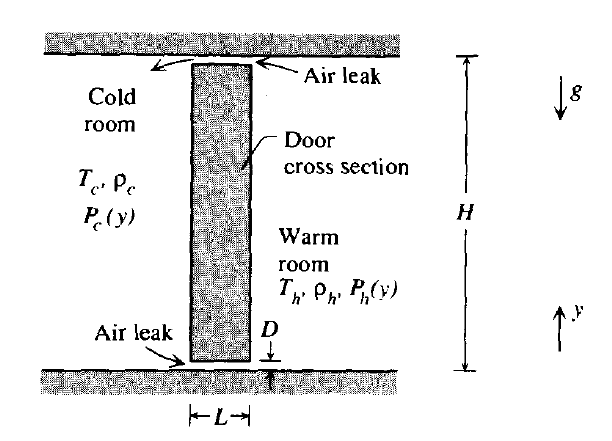
\includegraphics[width=.65\textwidth]{Figures/1_1}
	\caption{Diagrama de fluxo de ar entre volume quente e frio}
\end{figure}


\textbf{Desenvolvimento} 

O intercambio do calor entre o ar e a garrafa obedece ao equilíbrio da primeira lei da termodinâmica onde

\begin{equation}
	\begin{aligned}
		\dot{m} C_{p} \frac{dT}{dt} = hA(T_{s}-T_{inf})
	\end{aligned}
\end{equation}

Onde $h$ é o coeficiente de trasnferencia de calor, $A  (A= 2\pi rH + 2\pi r^{2})$ é a área superficial do cilindoO objetivo é encontrar uma relação entre o tempo de resfriamento e a troca de calor convectiva (lado direito da equação) para as posições 1 e 2. Considerando que o calor removido em ambos os arranjos é o mesmo

\begin{equation}
	\begin{aligned}
		Q_{1} = Q_{2}
	\end{aligned}
\end{equation}

\begin{equation}
	\begin{aligned}
		h_{1}A_{1}(T_{s}-T_{inf})t_{1} = h_{2}A_{2}(T_{s}-T_{inf})t_{2}
	\end{aligned}
\end{equation}

\begin{equation}
	\begin{aligned}
		\frac{t_{1} }{t_{2}}= \frac{h_{2}A_{2}}{h_{1}A_{1}}
	\end{aligned}
\end{equation}

Para análise de escala, a área do cilindro na posição vertical e horizontal é proporcional a $H$

\begin{equation}
	\begin{aligned}
		A \sim H \ \ ; \ \ H_{1} = 5H_{2}
	\end{aligned}
\end{equation}

Pela definição do número de Nusselt

\begin{equation}
	\begin{aligned}
		Nu_{H} = \left( \frac{hH}{k}\right) \sim Ra^{\frac{1}{4}}
	\end{aligned}
\end{equation}

A equaçao 4 fica então

\begin{equation}
	\begin{aligned}
		Nu_{H} = \left( \frac{hH}{k}\right) \sim Ra^{\frac{1}{4}}
	\end{aligned}
\end{equation}




















\begin{thebibliography}{999}
	
	
	\bibitem{abejan}
	Adrian Bejan,
	Convection Heat Transfer.
	Durham, North Carolina,
	3rd Edition,
	2004.
	
	\bibitem{naraghi}
	Adrian Bejan,
	Shape and structure from engineering to nature.
	Cambridge University, USA.
	2000.
	
\end{thebibliography}



\end{document}





